
\documentclass[fleqn,addpoints]{exam}

\usepackage{graphicx}
\usepackage{float}
\usepackage{amsmath}
\usepackage{cancel}
\usepackage{polynom}
\usepackage{caption}

\printanswers

\ifprintanswers \usepackage{2in1, lscape} \fi

\title{Math 115 Homework 7}
\date{November 13, 2010}

\begin{document}

\maketitle
 
\section{From the Book}

\vspace{0.2 cm}

Read section 1.12.
 
\begin{itemize}
  \item p. 82: 12-13
  \item p. 100: 1-10, 14-15, 17-19, 21-22
\end{itemize}

\section{Page 82}
\begin{itemize}
\item[12 a]
\begin{figure}[H]
  \centering
  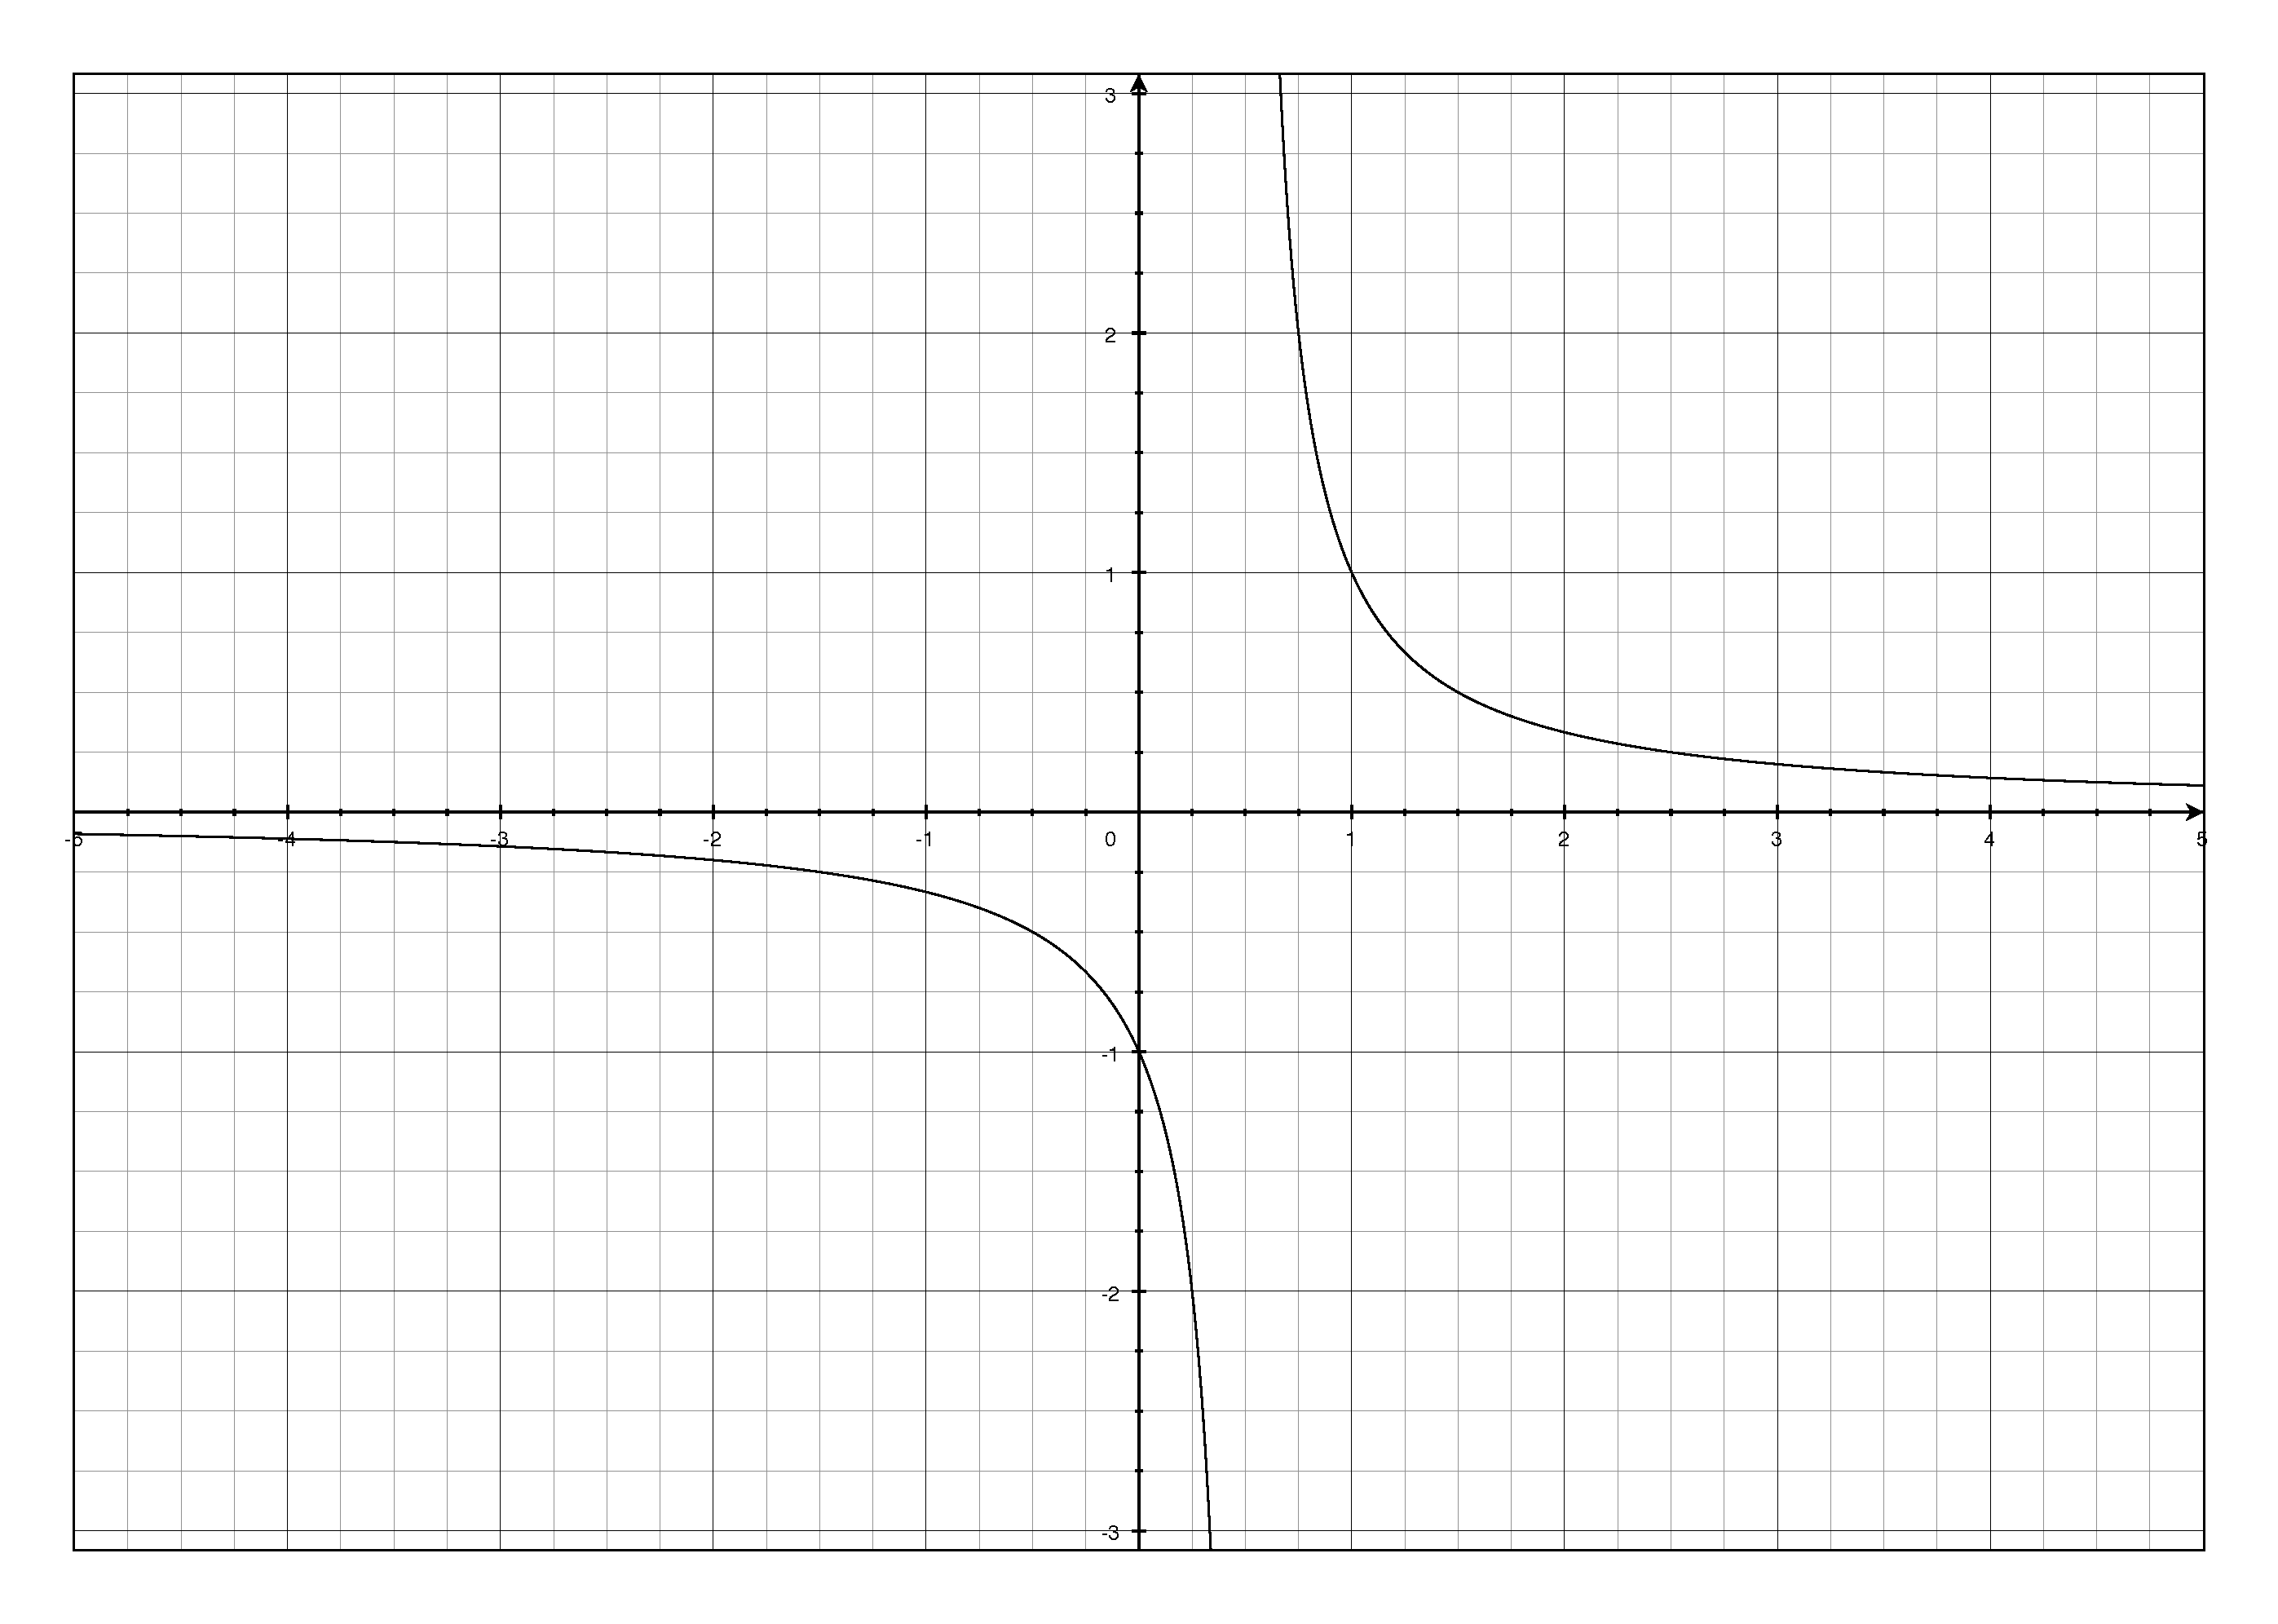
\includegraphics[width=7cm,height=5cm]{p82-12a.eps}
  \caption*{Problem 12 a: $f(x) = \dfrac{1}{2x-1}$}
\end{figure}

\item[12 b]
\begin{figure}[H]
  \centering
  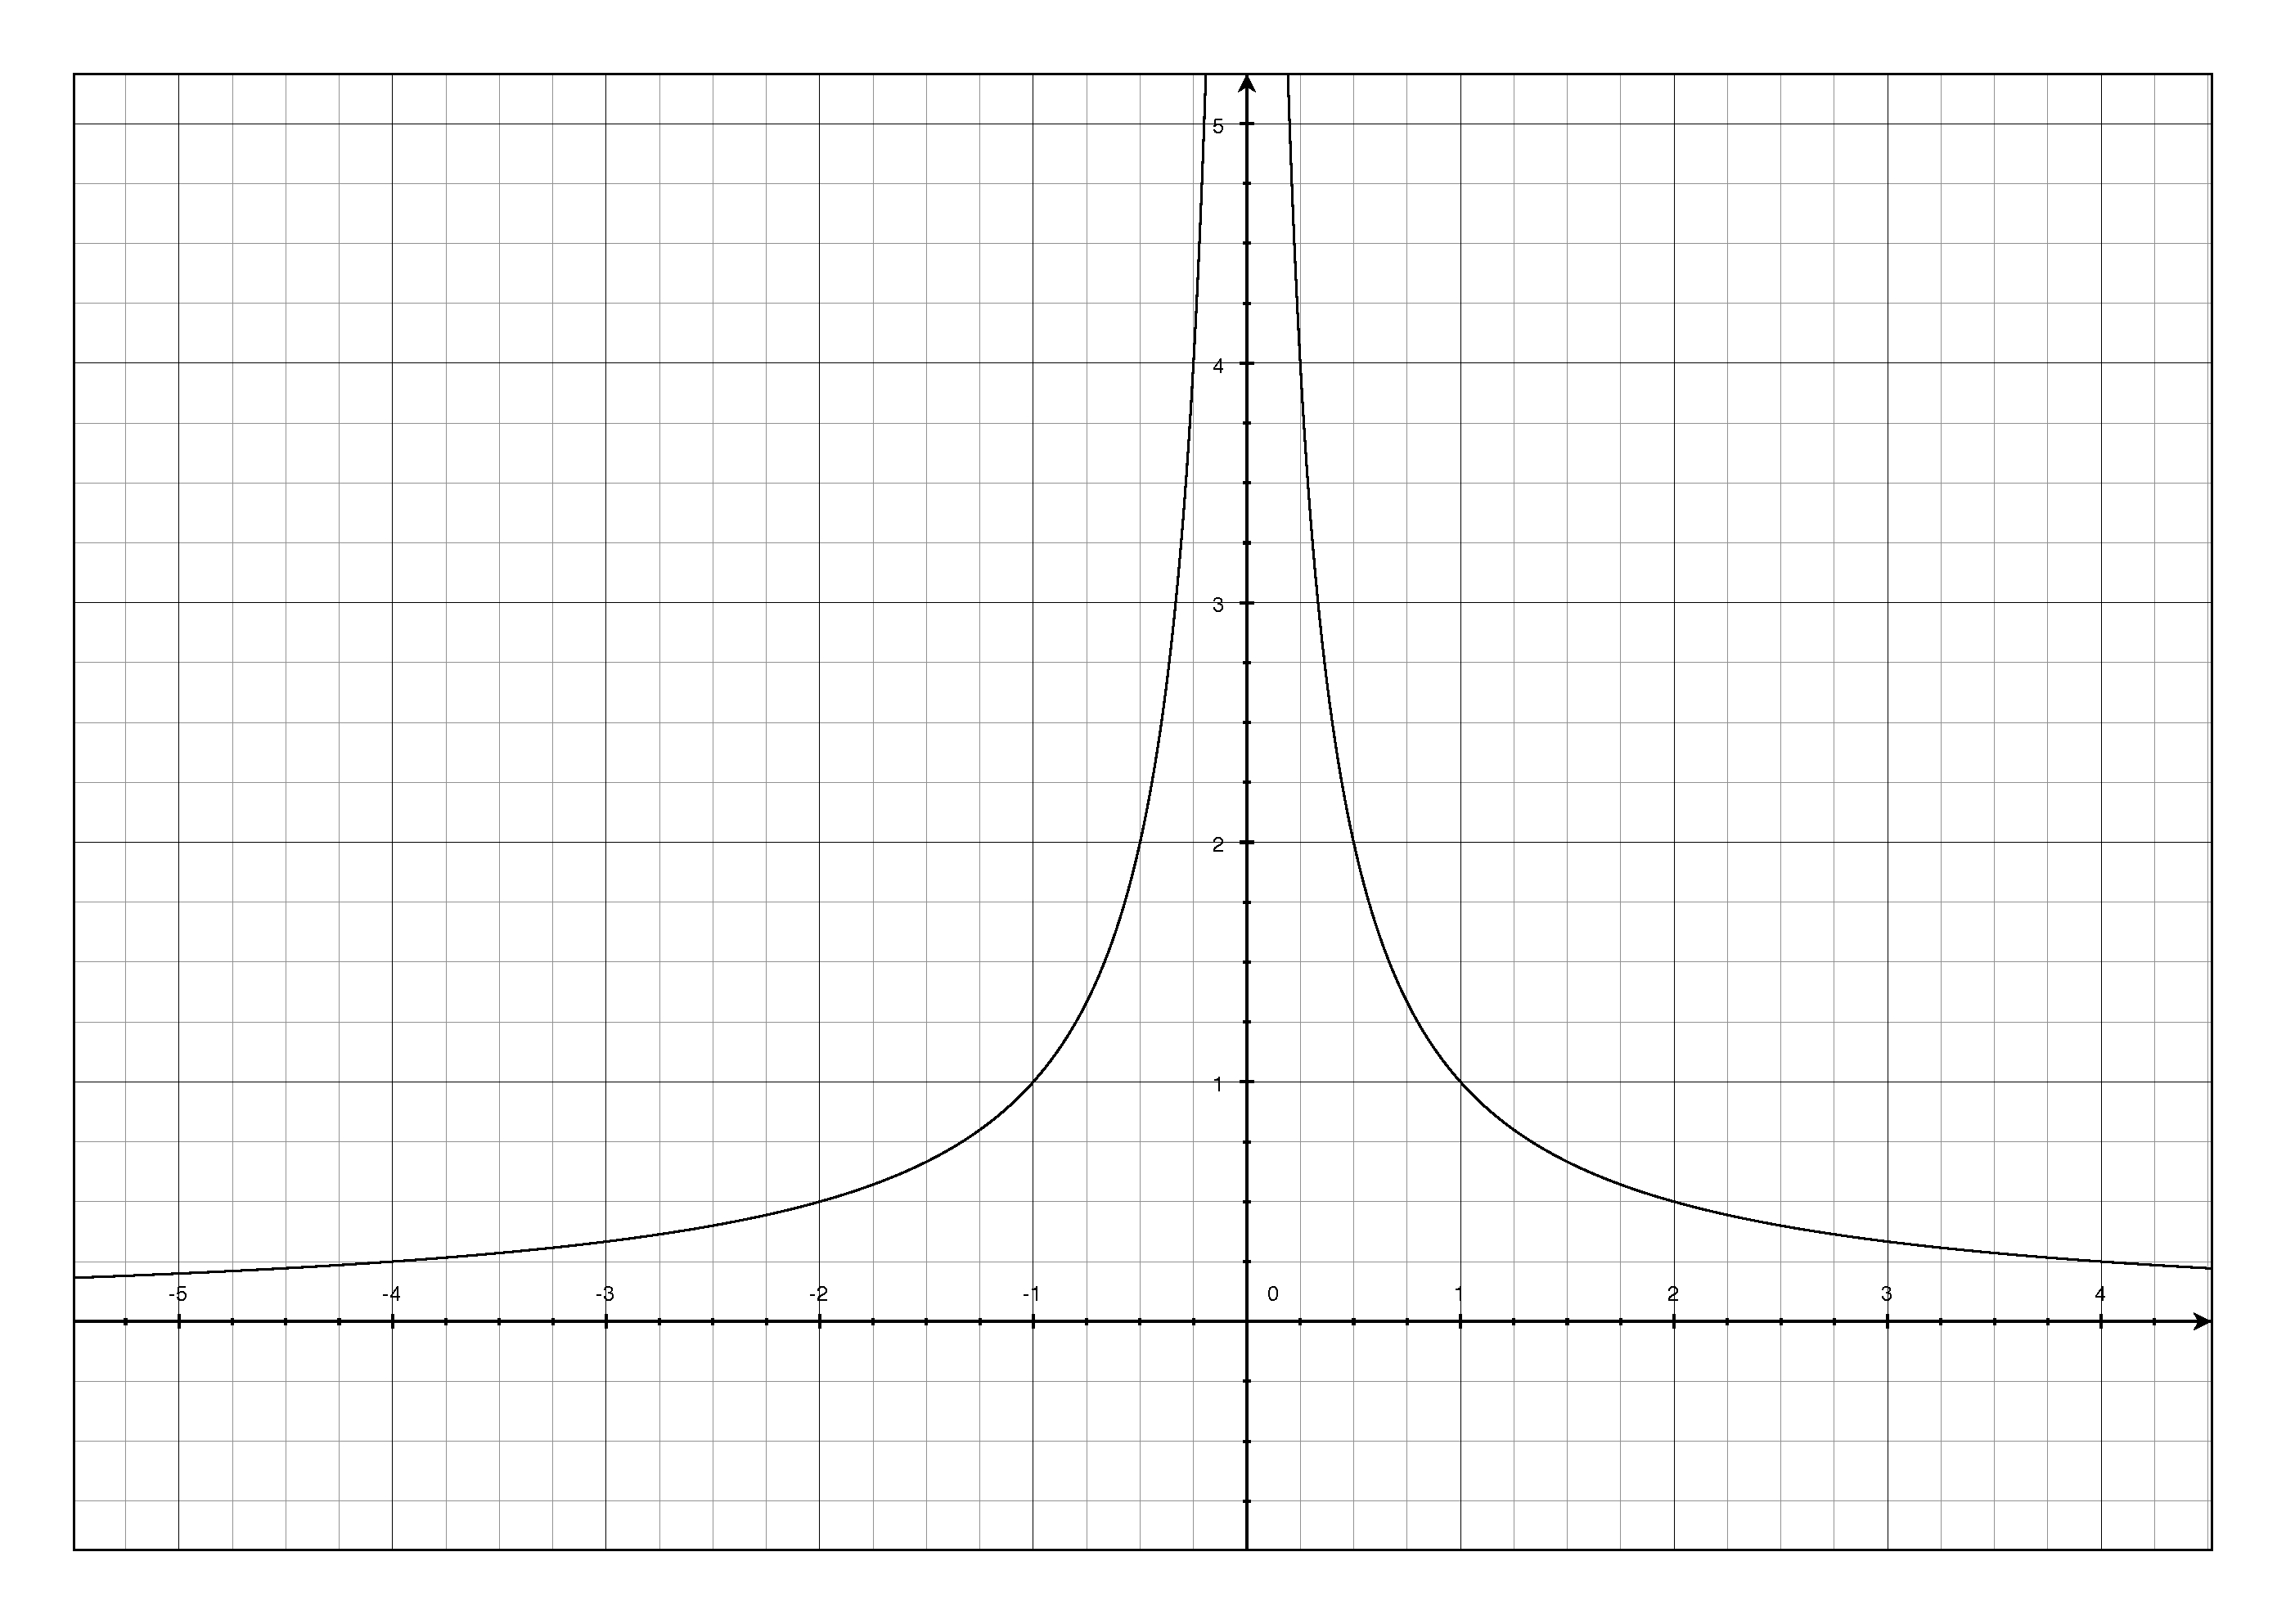
\includegraphics[width=7cm,height=5cm]{p82-12b.eps}
  \caption*{Problem 12 b: $f(x) = \dfrac{1}{|x|}$}
\end{figure}

\item[12 c]
\begin{figure}[H]
  \centering
  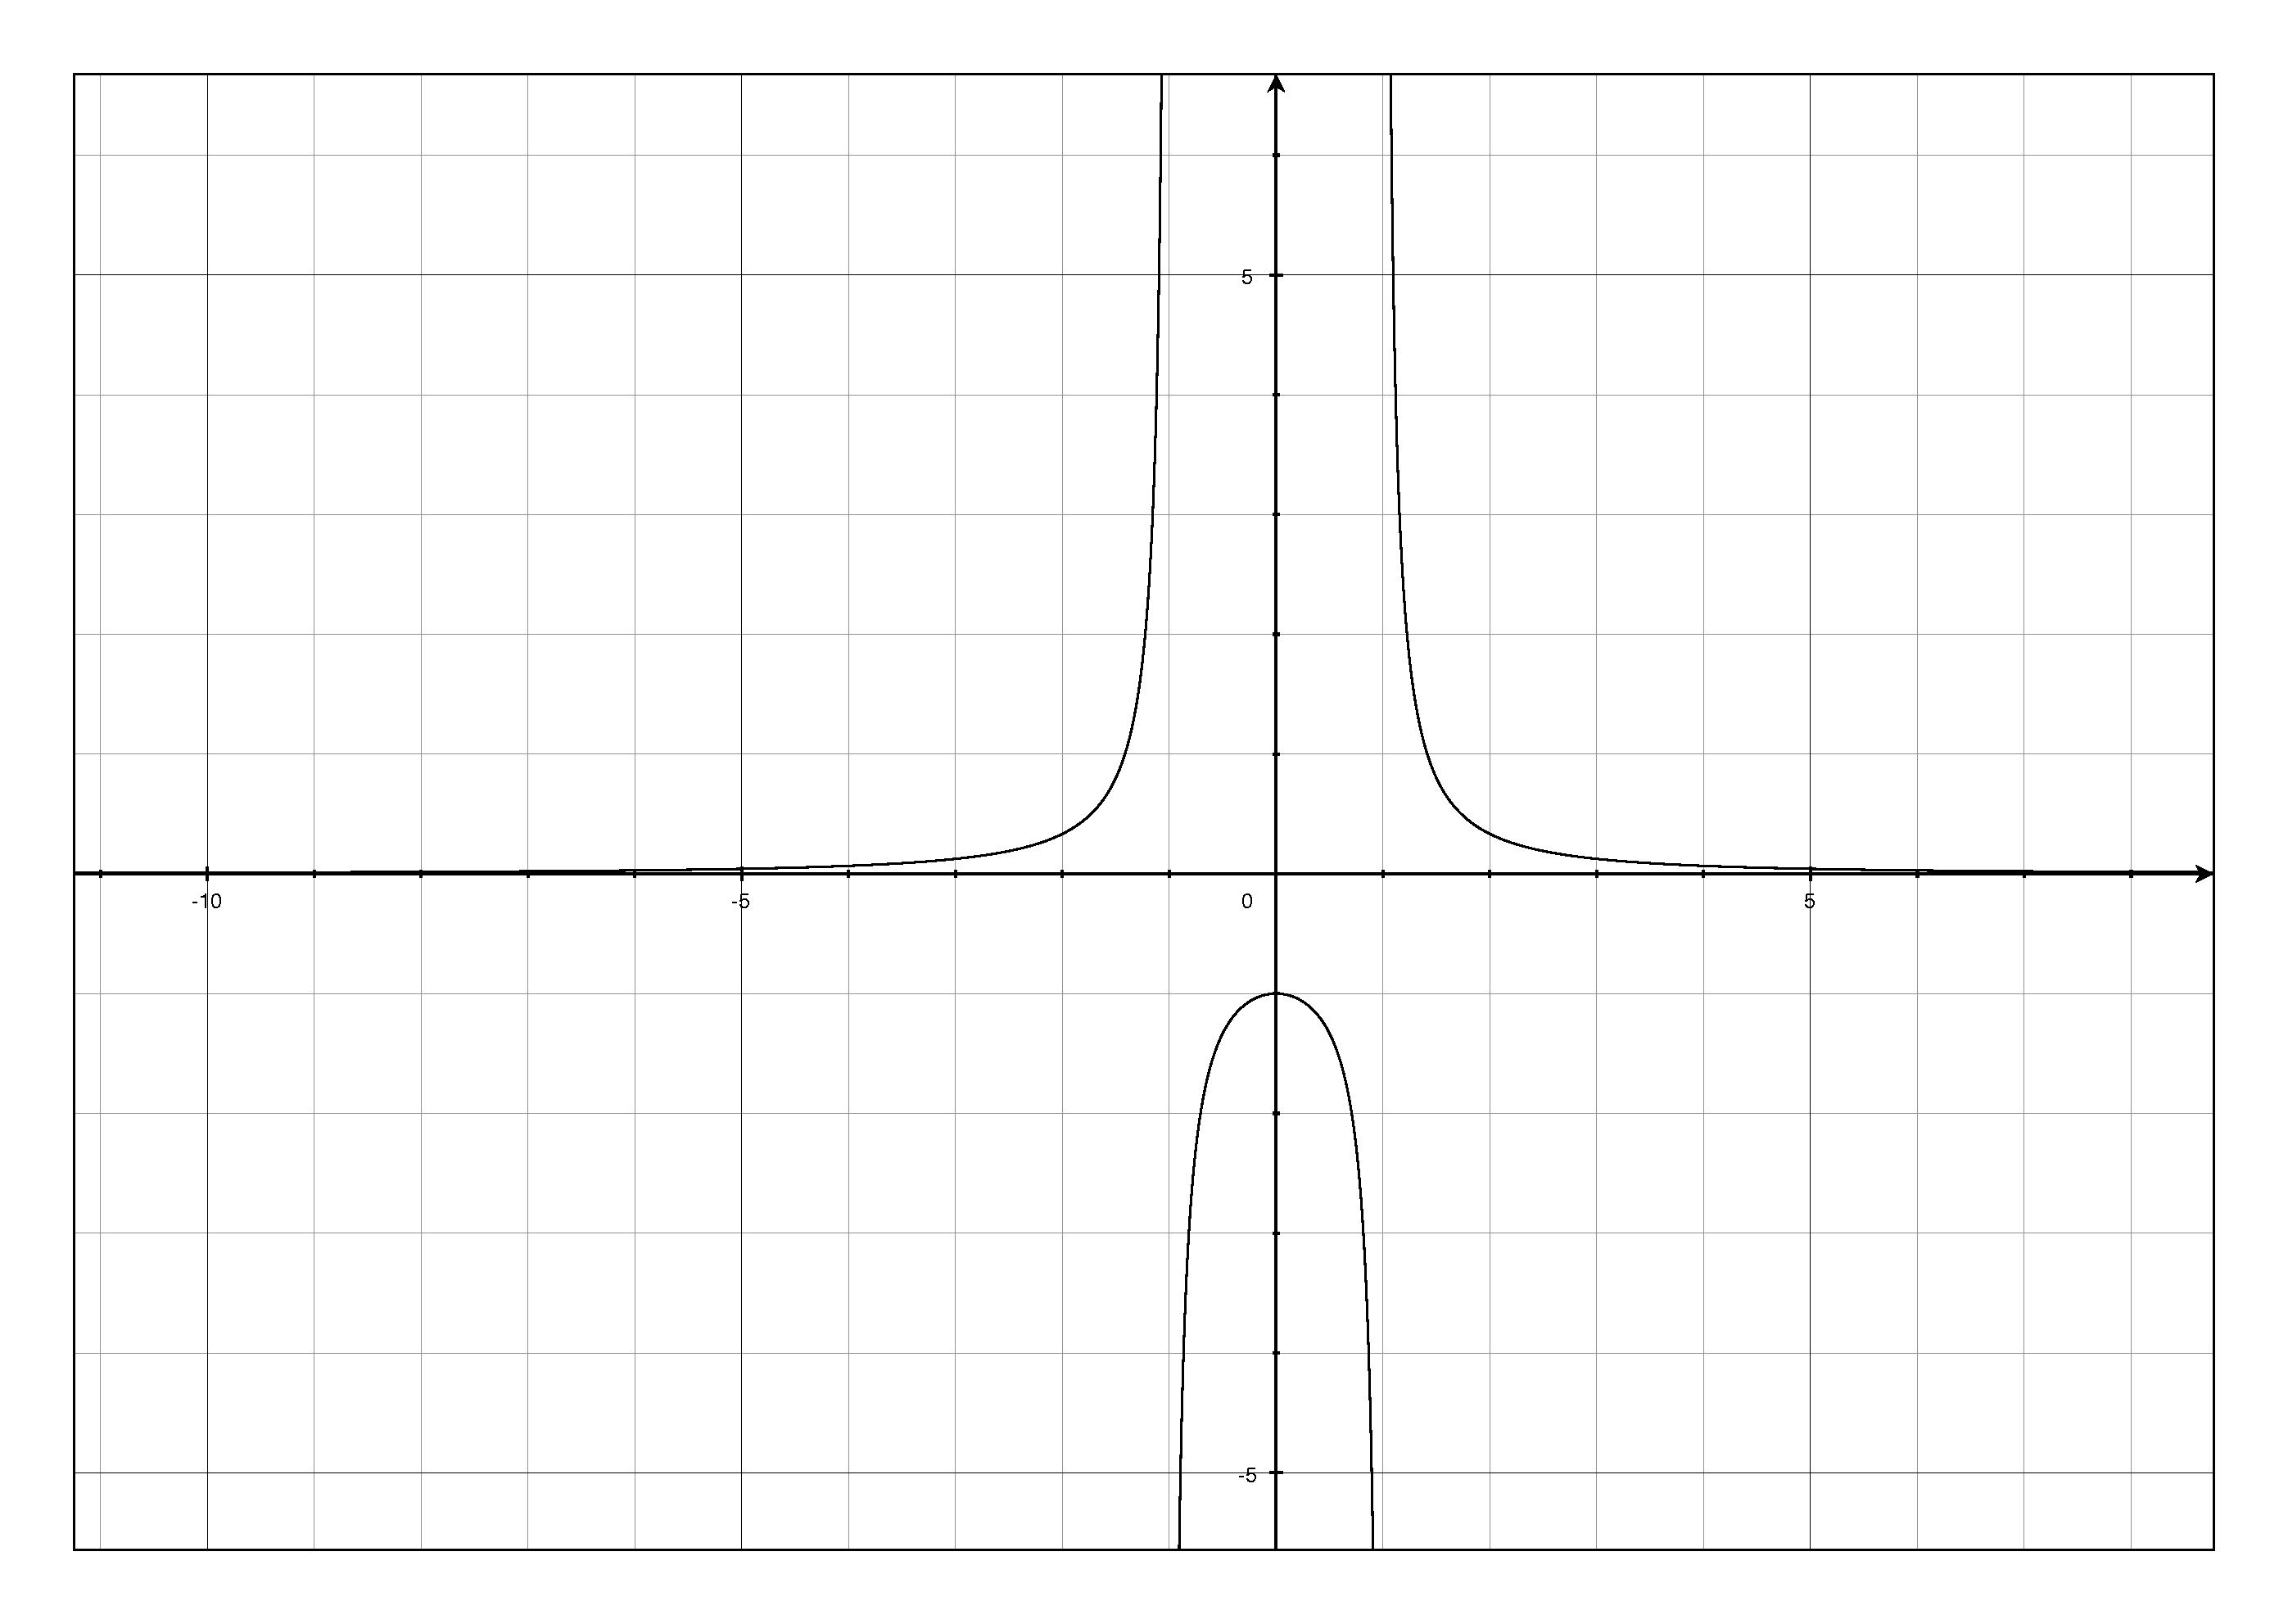
\includegraphics[width=7cm,height=5cm]{p82-12c.eps}
  \caption*{Problem 12 c: $f(x) = \dfrac{1}{x^2-1}$}
\end{figure}

\item[12 d]
\begin{figure}[H]
  \centering
  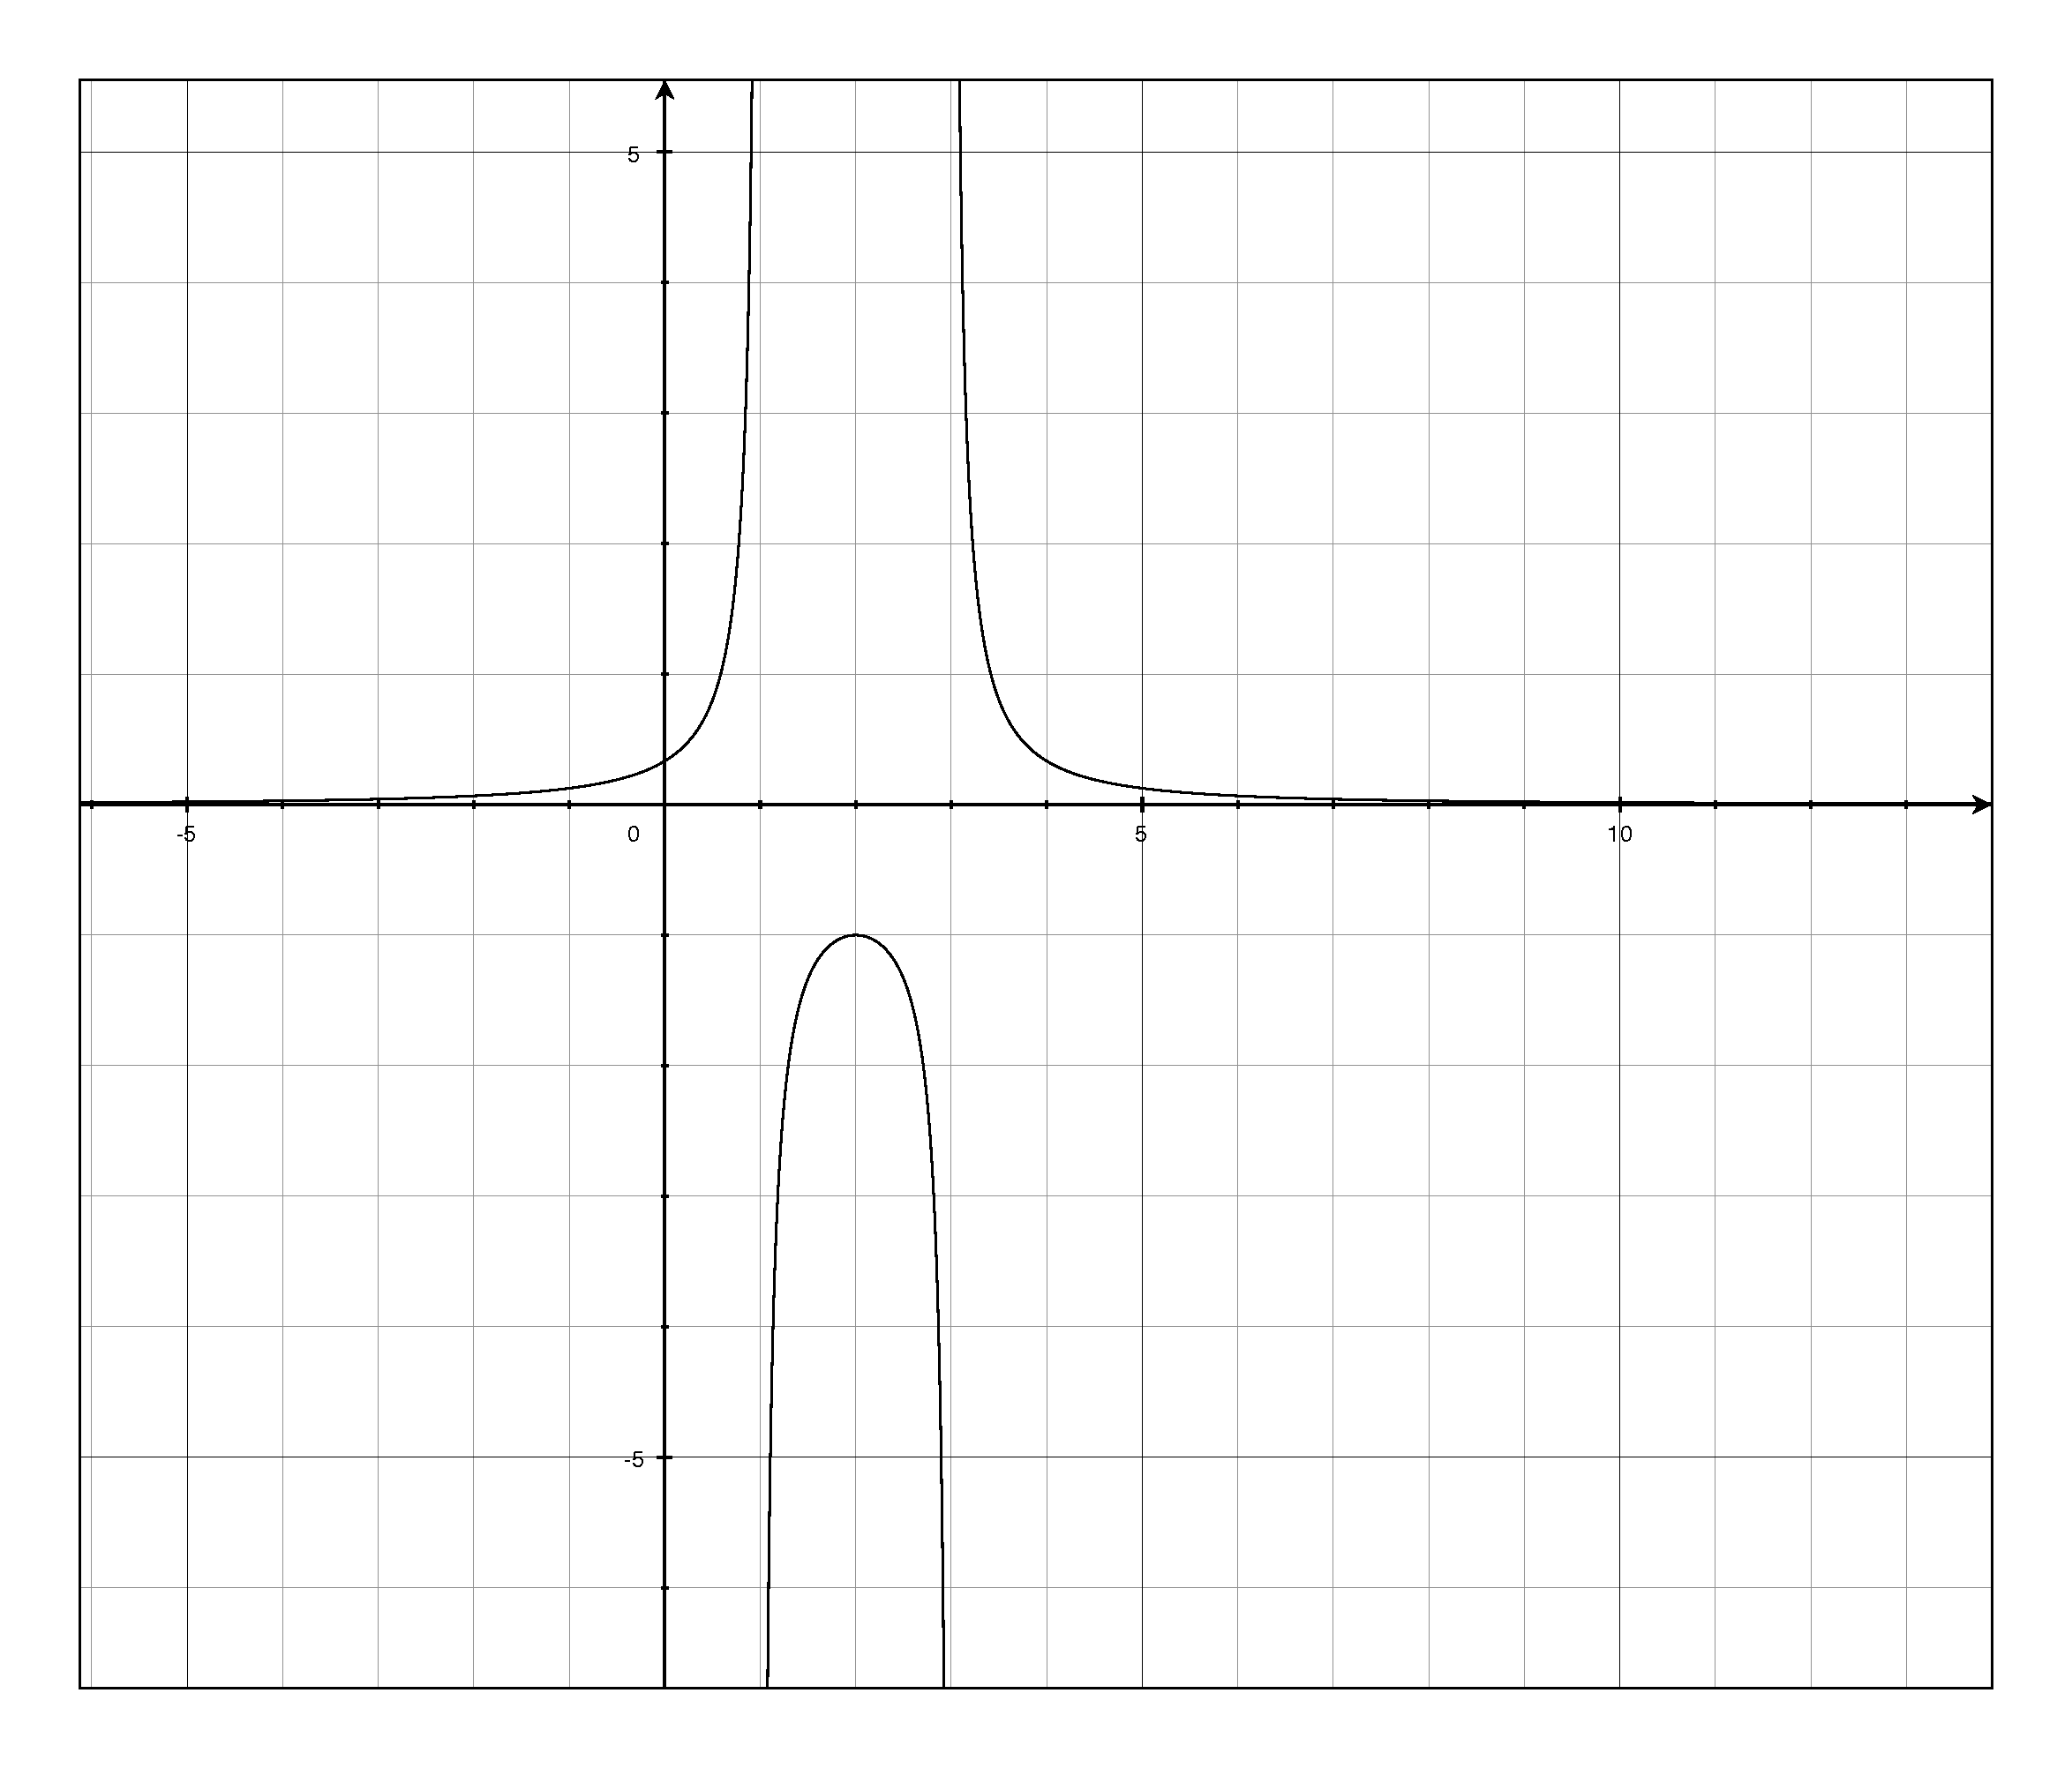
\includegraphics[width=7cm,height=5cm]{p82-12d.eps}
  \caption*{Problem 12 d: $f(x) = \dfrac{1}{x^2-4x+3}$}
\end{figure}

\item[13 a]
\begin{figure}[H]
  \centering
  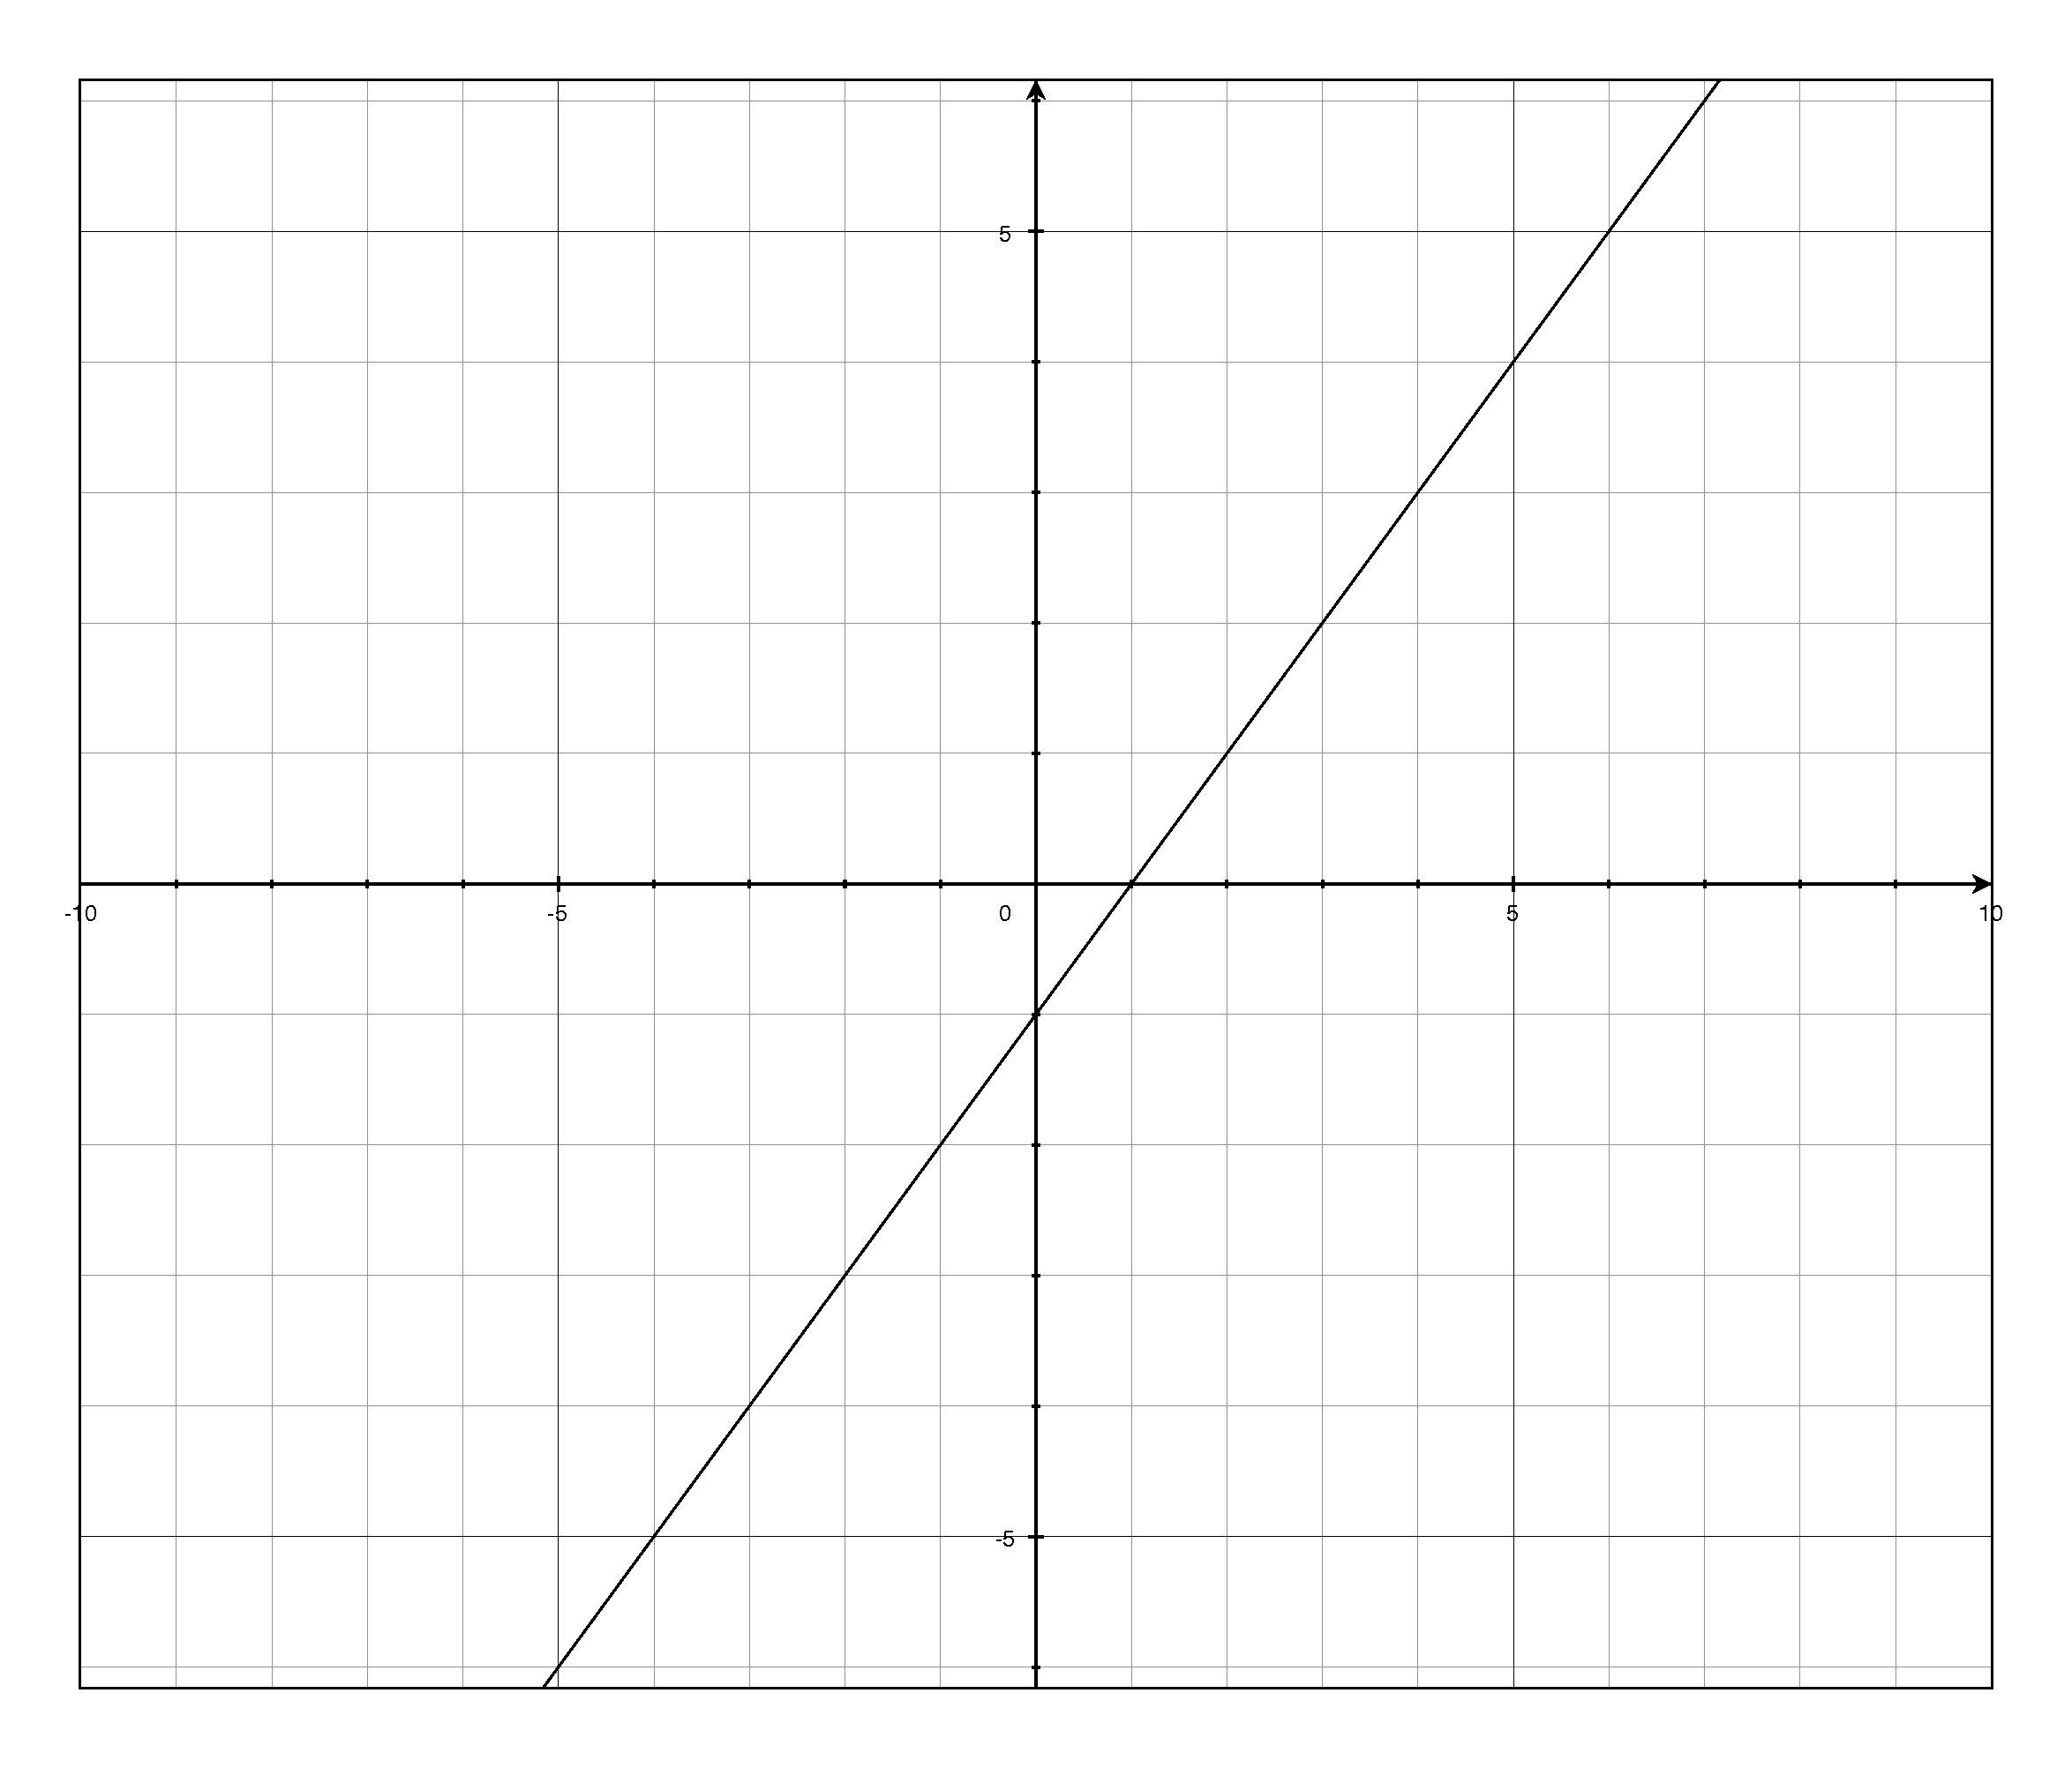
\includegraphics[width=7cm,height=5cm]{p82-13a.eps}
  \caption*{Problem 13 a: $f(x) = x-1$}
\end{figure}

\item[13 b]
\begin{figure}[H]
  \centering
  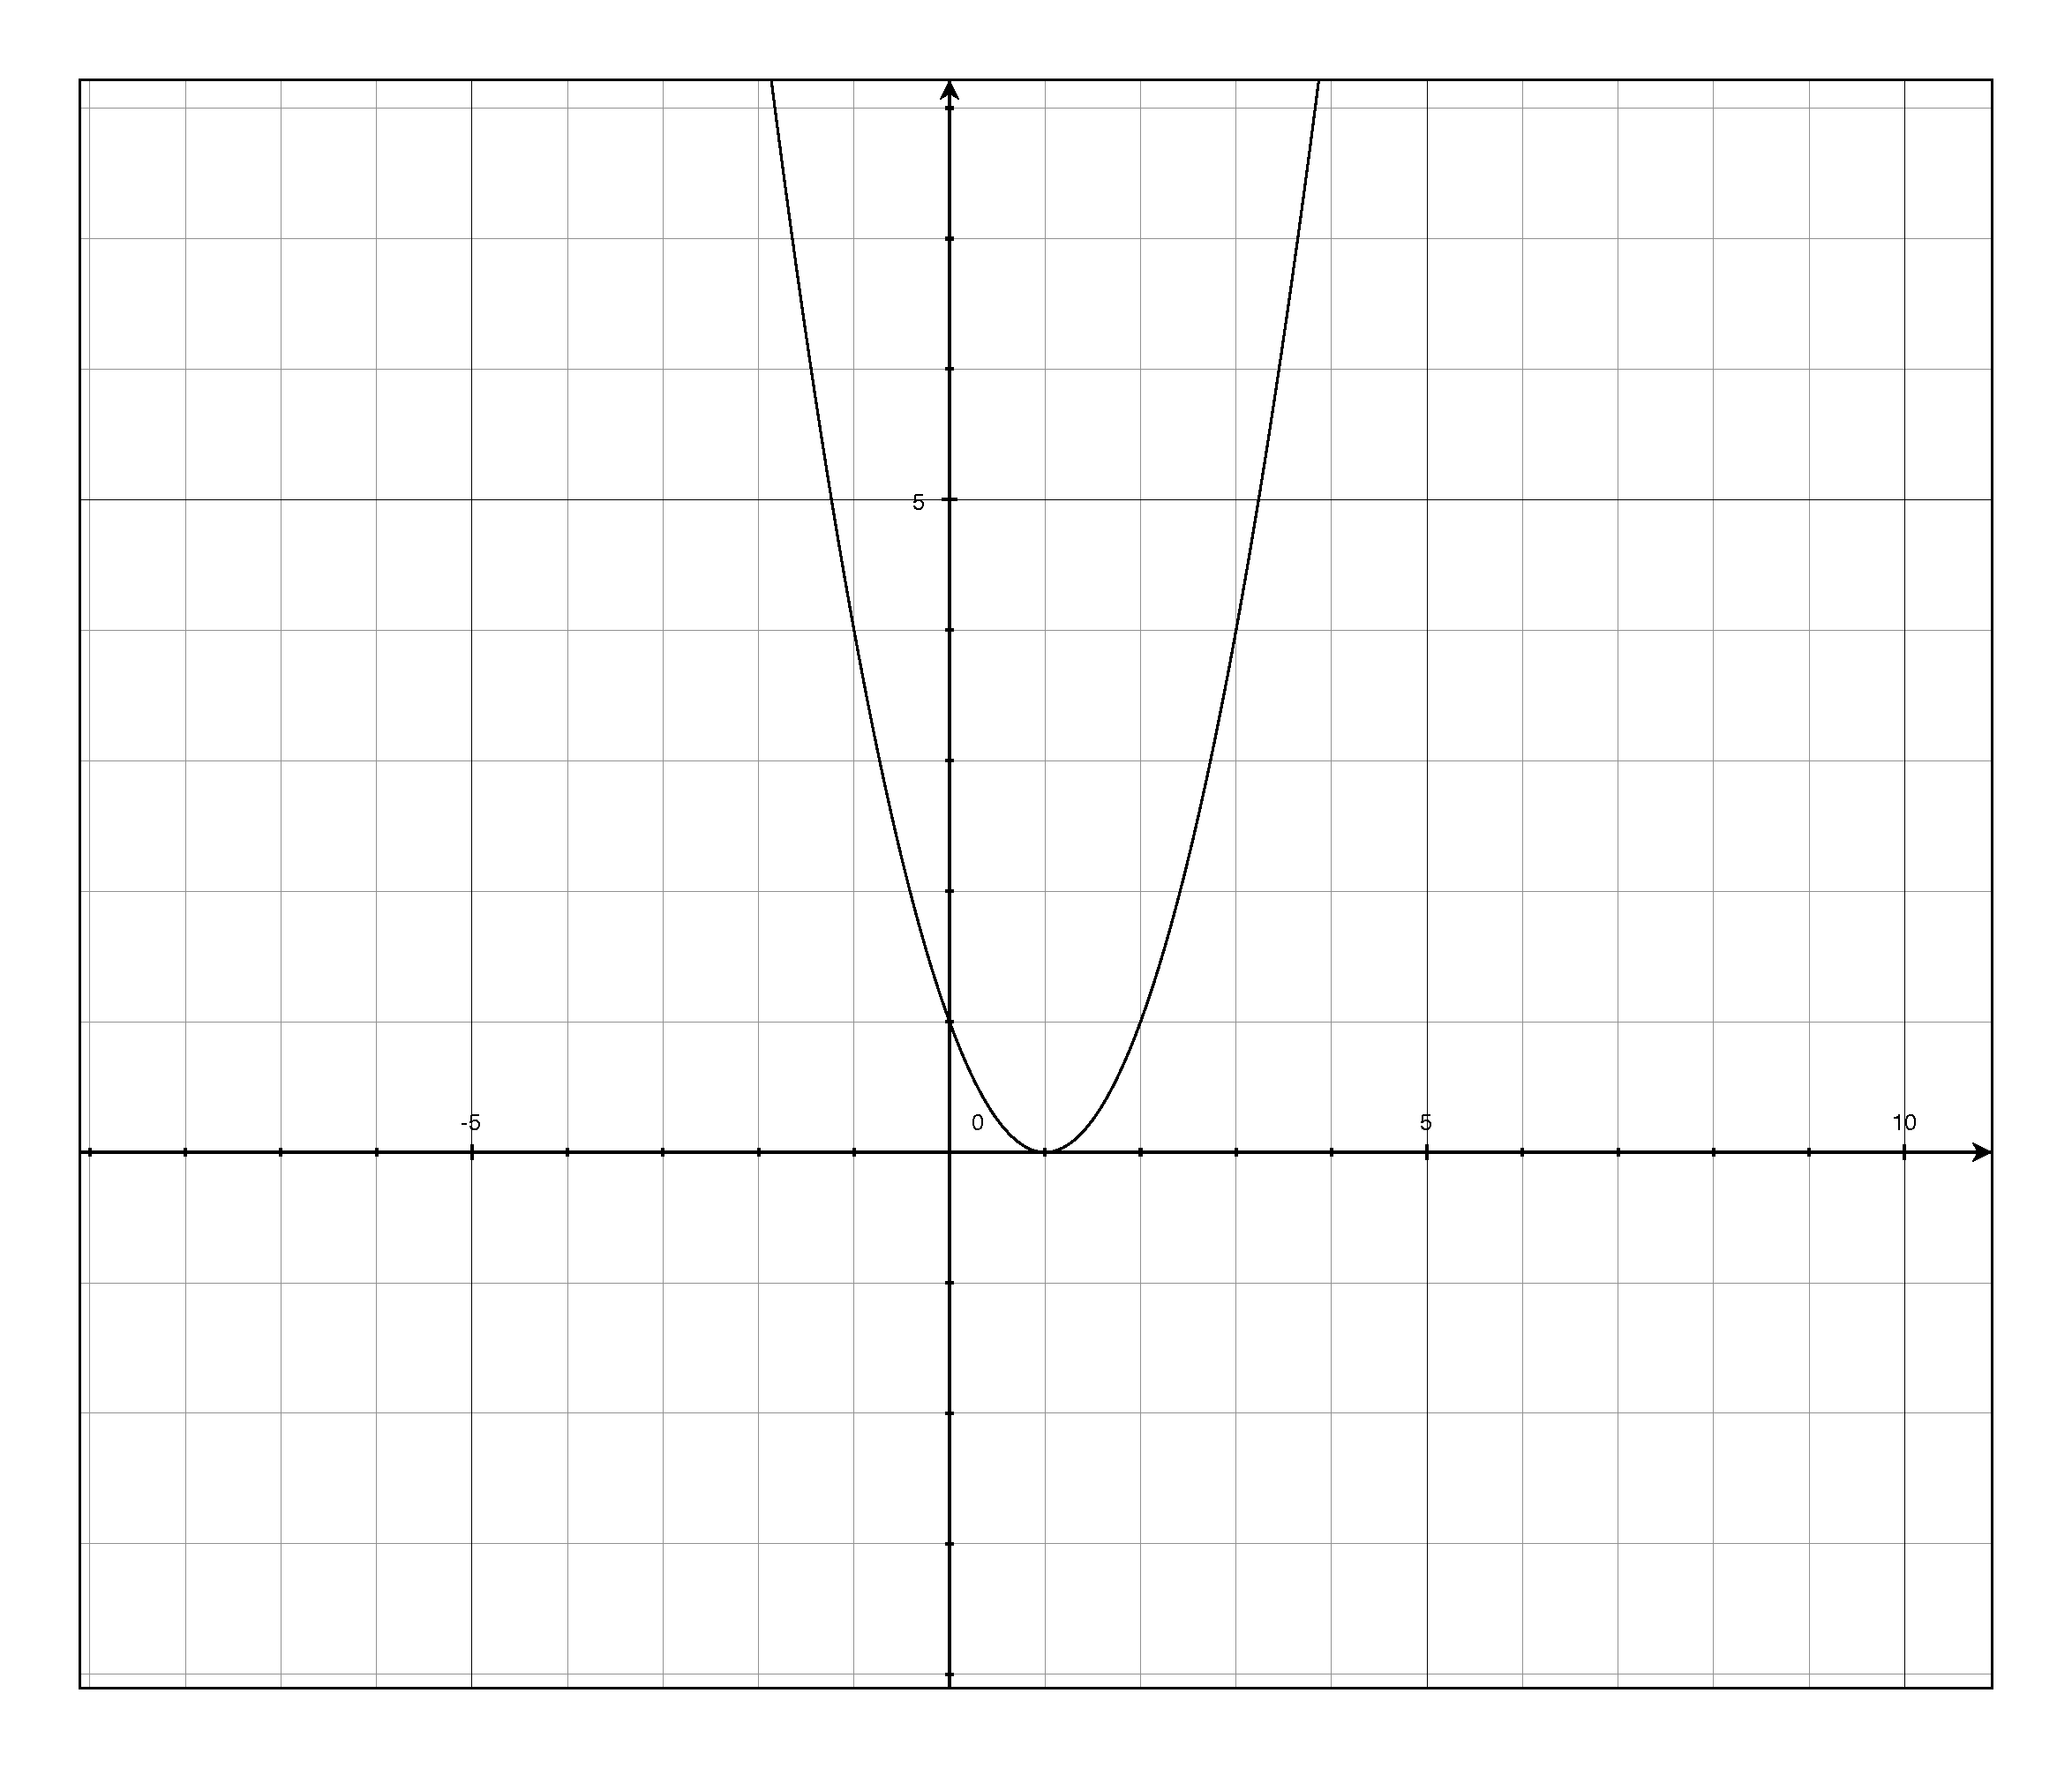
\includegraphics[width=7cm,height=5cm]{p82-13b.eps}
  \caption*{Problem 13 b: $f(x) = (x-1)^2$}
\end{figure}

\item[13 c]
\begin{figure}[H]
  \centering
  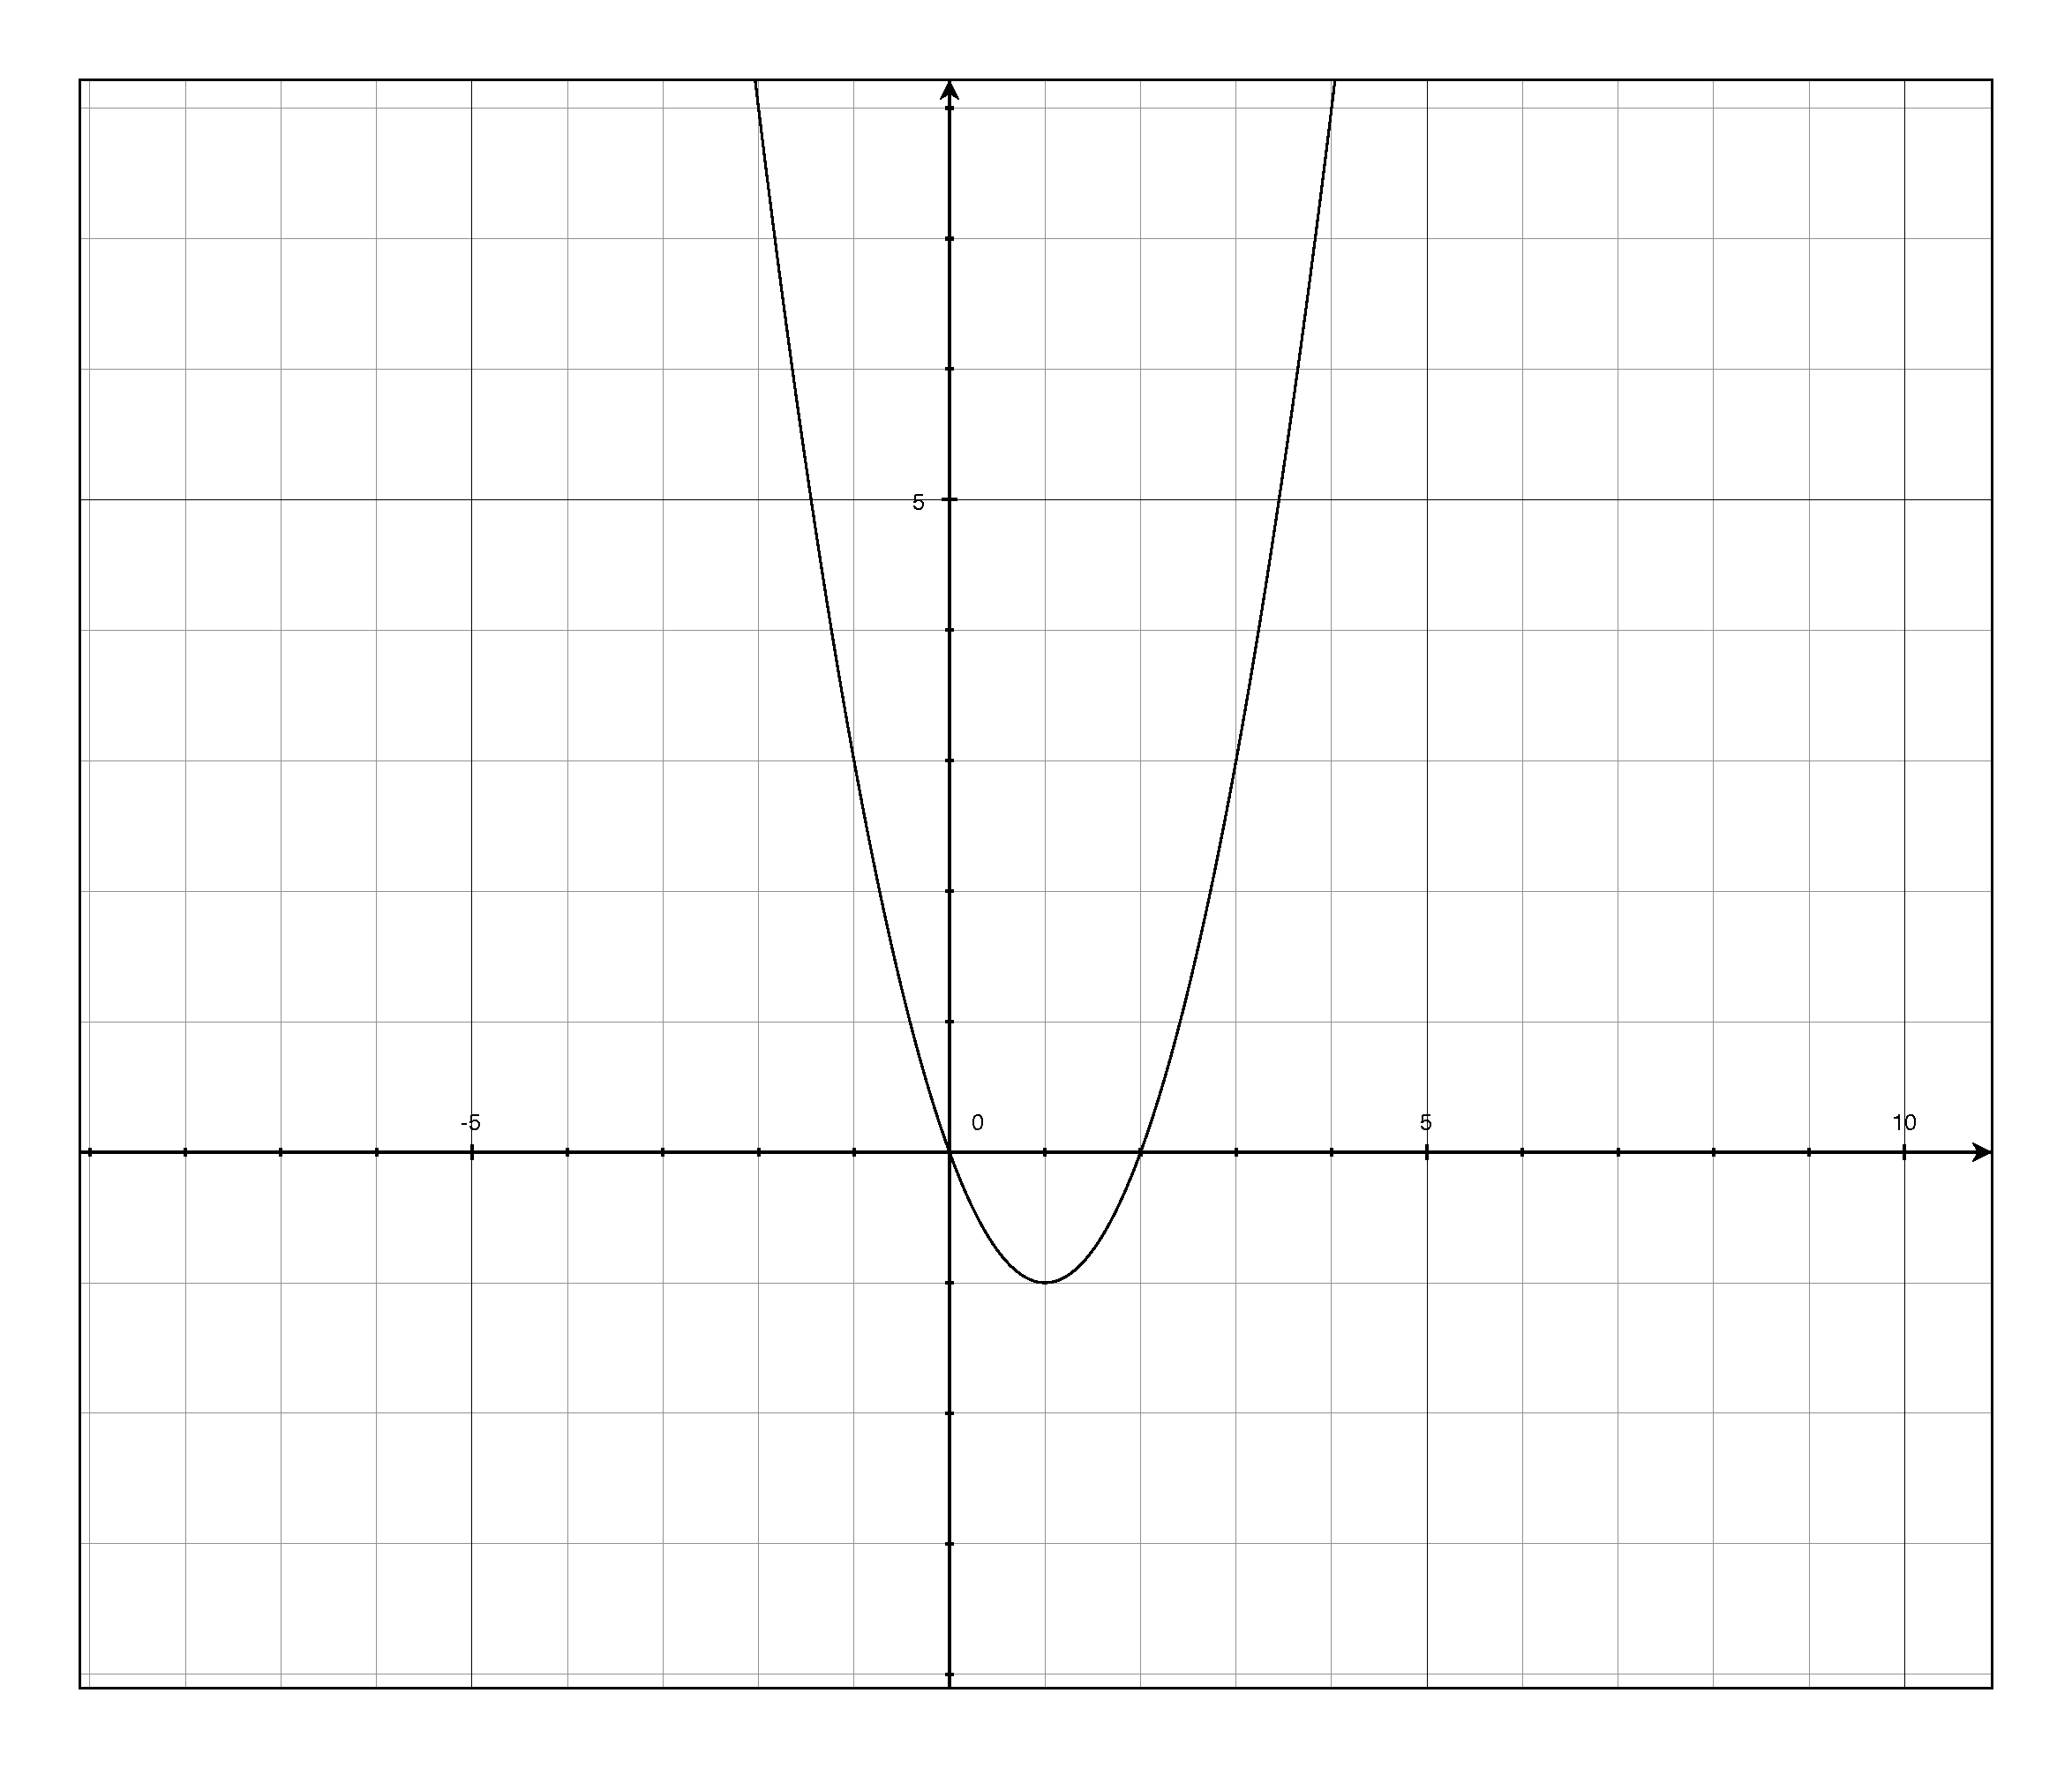
\includegraphics[width=7cm,height=5cm]{p82-13c.eps}
  \caption*{Problem 13 c: $f(x) = x^2 - 2x$}
\end{figure}

\item[13 d]
\begin{figure}[H]
  \centering
  \includegraphics[width=7cm,height=5cm]{p82-13d.eps}
  \caption*{Problem 13 d: $f(x) = |x^2 - 2x|$}
\end{figure}

\item[13 e]
\begin{figure}[H]
  \centering
  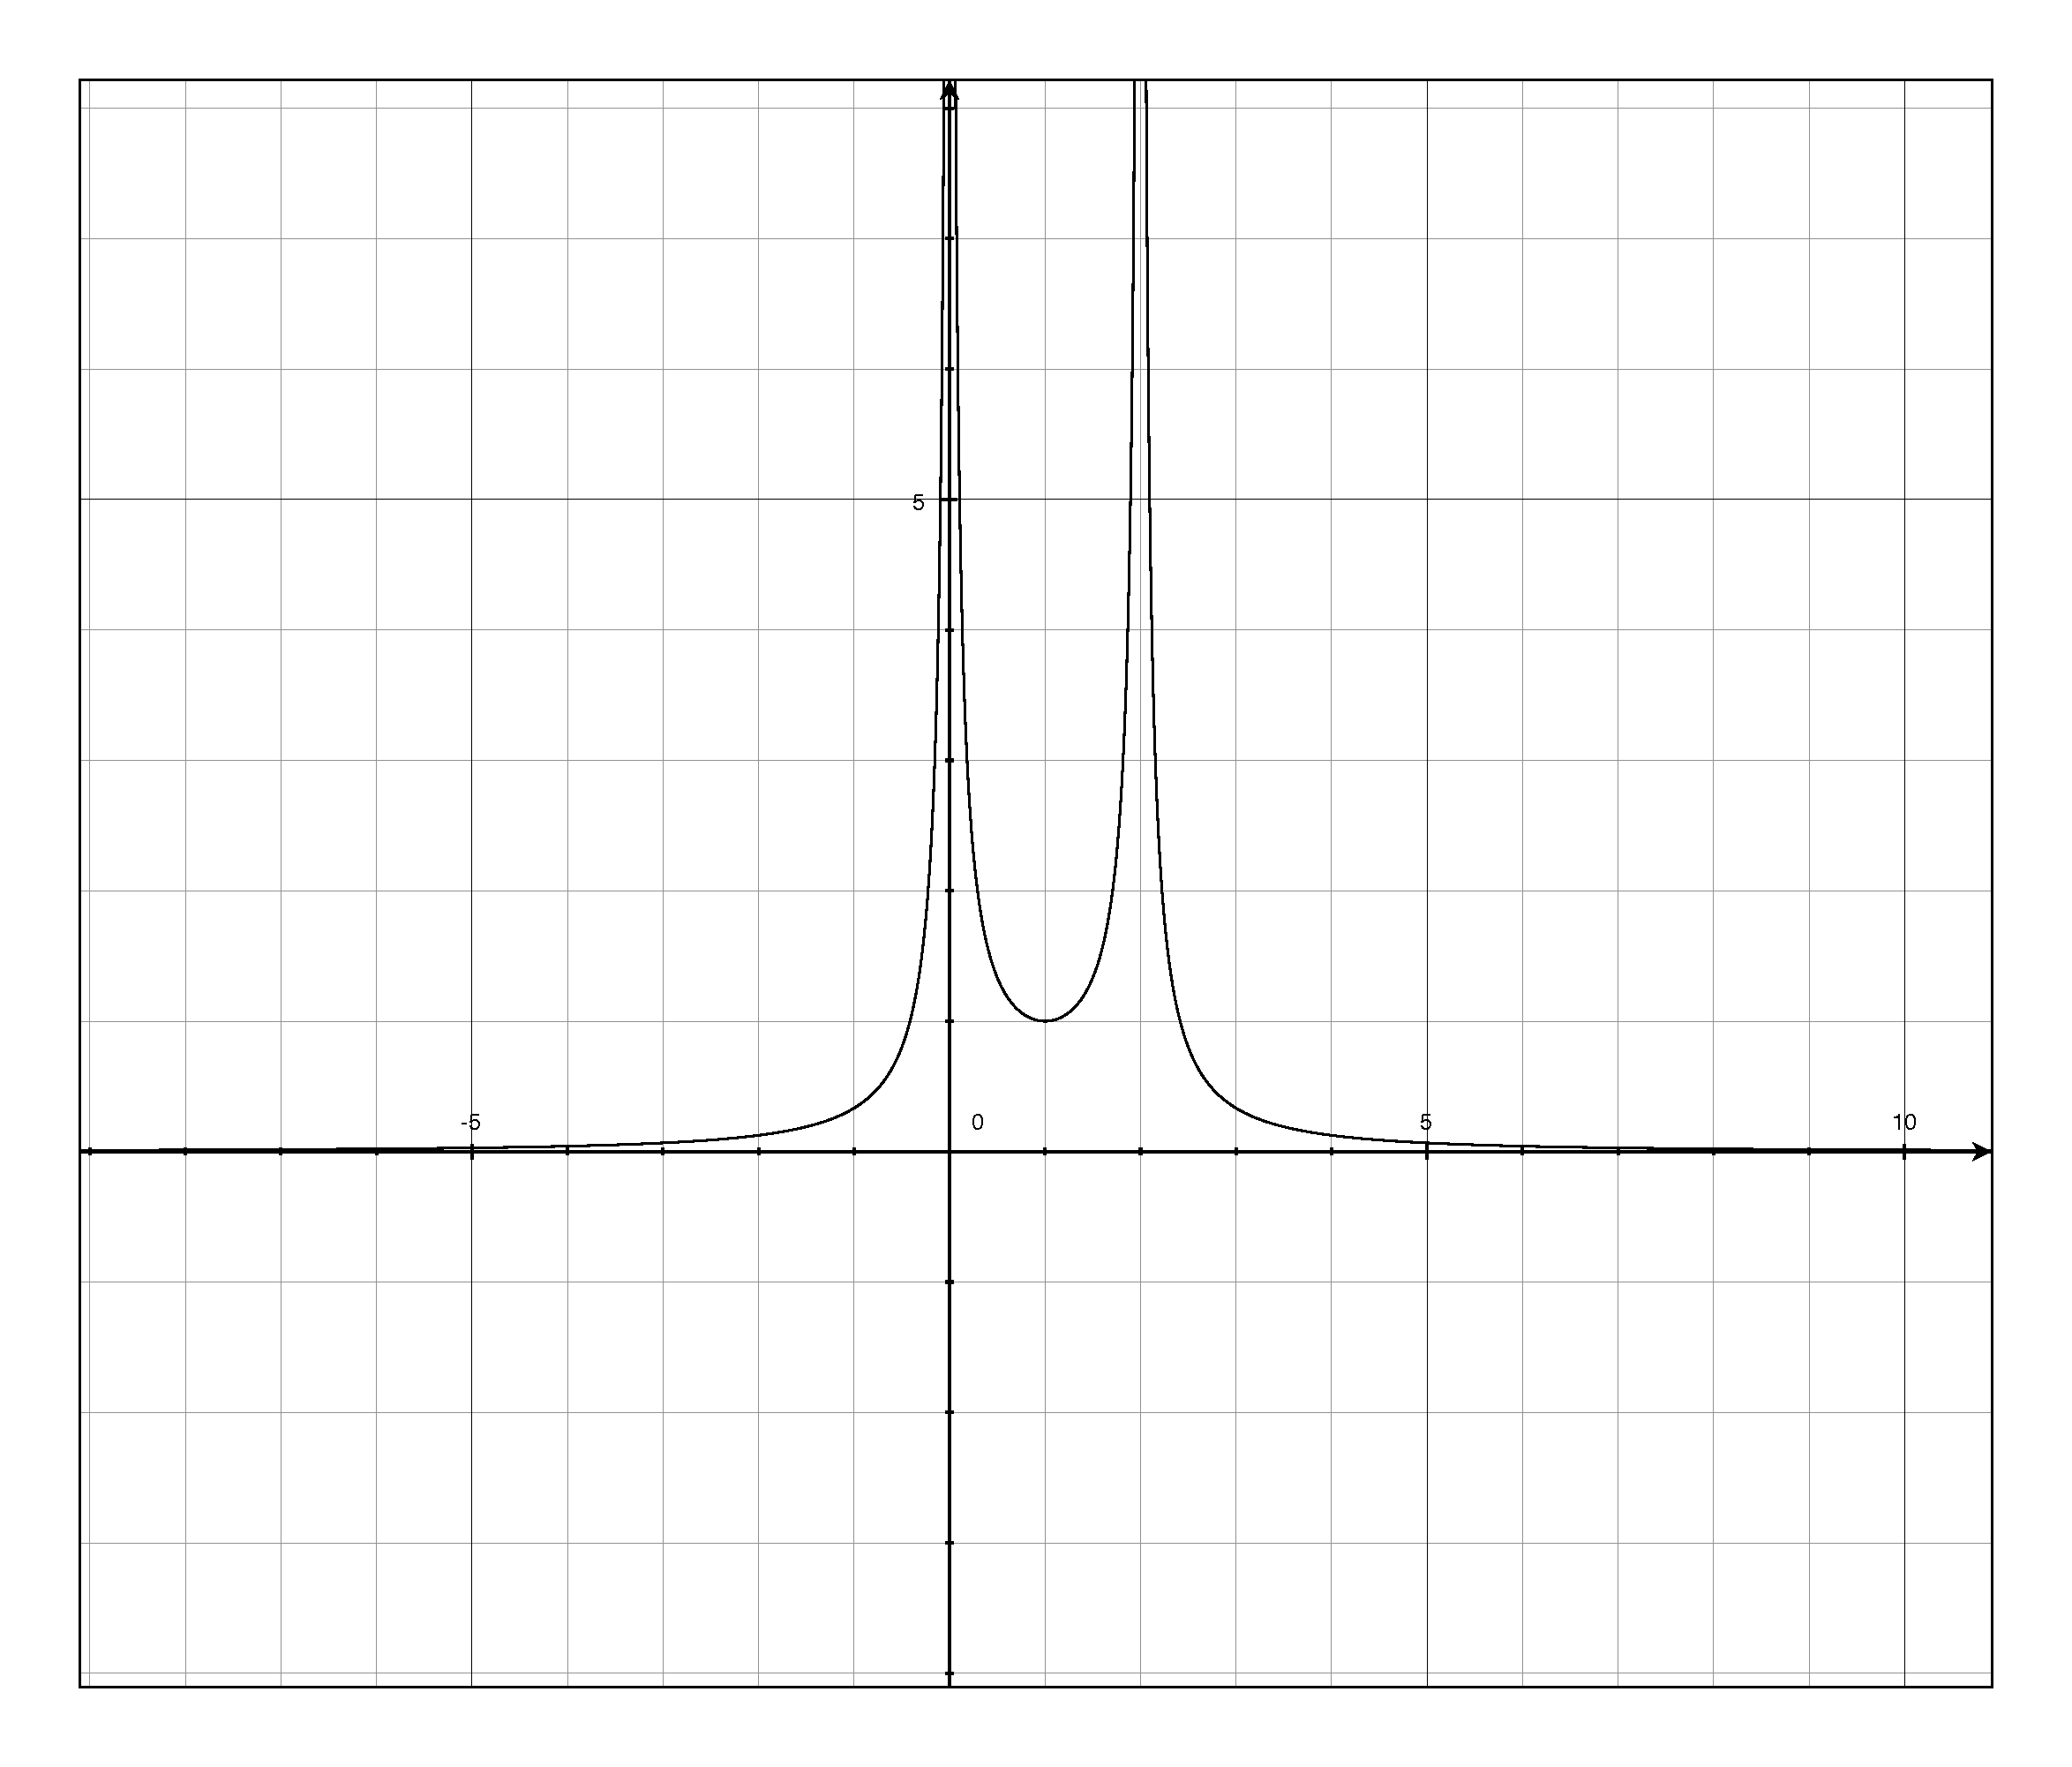
\includegraphics[width=7cm,height=5cm]{p82-13e.eps}
  \caption*{Problem 13 e: $f(x) = \dfrac{1}{|x^2 - 2x|}$}
\end{figure}

\item[13 f]
\begin{figure}[H]
  \centering
  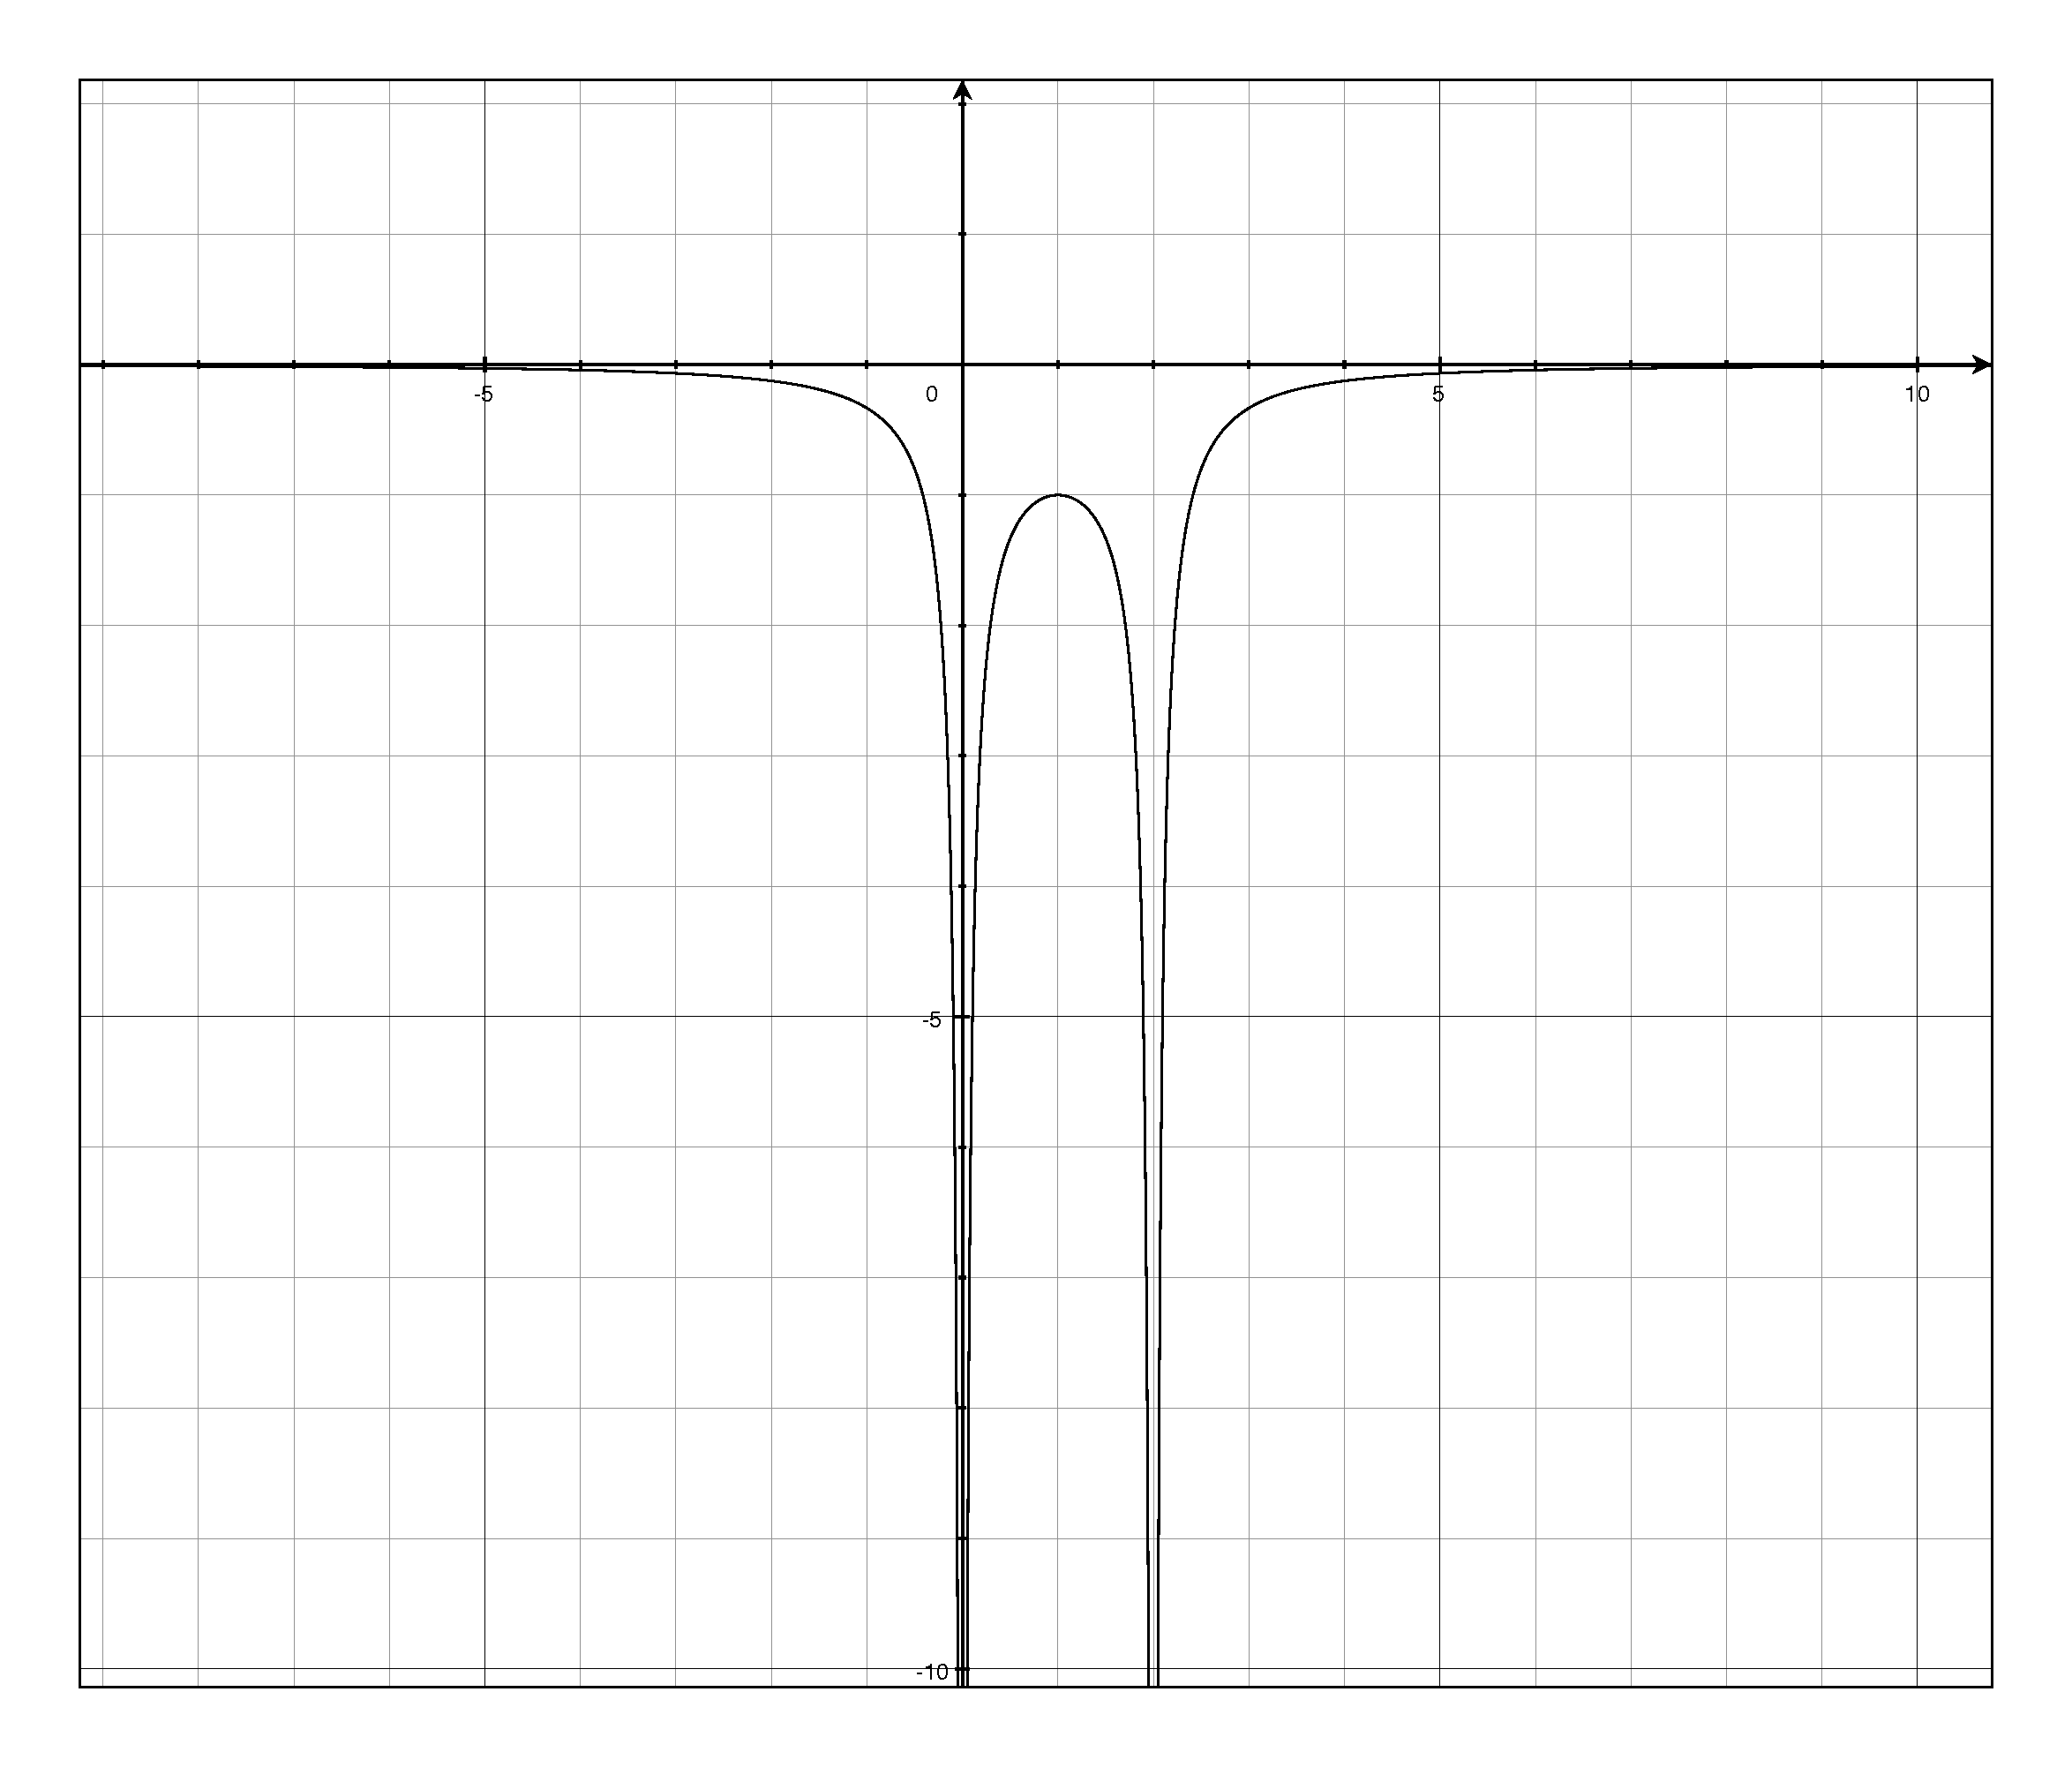
\includegraphics[width=7cm,height=5cm]{p82-13f.eps}
  \caption*{Problem 13 f: $f(x) = \dfrac{-1}{|x^2 - 2x|}$}
\end{figure}


\end{itemize}

\section{Page 100}

Using the horizontal line test, numbers 1, 4, and 6 are one-to-one.

\begin{itemize}
\item[7]
$f(x)$ is one-to-one:
\begin{align*}
  3x_1 - 4 &= 3x_2 - 4 \\
  3x_1 &= 3x_2 \\
  x_1 &= x_2 \\
\end{align*}

\item[8]
$f(x) = |x|$ is not one-to-one since for any value of $x$ other than 0, $f(x) = f(-x)$.

\item[9]
$f(x)$ is one-to-one:
\begin{align*}
  \sqrt{x_1 - 1} &= \sqrt{x_2 - 1} \\
  x_1 - 1 &= x_2 - 1 \\
  x_1 &= x_ 2 \\
\end{align*}

\item[10]
$f(x) = x^2 - 3x + 2$ is a parabola and so it is not one-to-one.

\item[17]
$f(x) = 2x-1$

$f(x)$ is one-to-one:
\begin{align*}
  2x_1 - 1 &= 2x_2 - 1 \\
  2x_1 &= 2x_2 \\
  x_1 &= x_2 \\
\end{align*}

Find $f^{-1}(x)$:
\begin{align*}
  y &= 2x-1 \\
  2x &= y + 1 \\
  x &= \frac{y+1}{2} \\
  \\
  f^{-1}(x) &= \frac{x+1}{2} \\
\end{align*}

\item[18]
$f(x) = \dfrac{4x-3}{2}$

$f(x)$ is one-to-one:
\begin{align*}
  \frac{4x_1-3}{2} &= \frac{4x_2-3}{2} \\
  4x_1-3 &= 4x_2 - 3 \\
  4x_1 &= 4x_2 \\
  x_1 &= x_2 \\
\end{align*}

find $f^{-1}(x)$:
\begin{align*}
  y &= \frac{4x-3}{2} \\
  2y &= 4x-3 \\
  x &= \frac{2y+3}{4}
  \\
  f^{-1}(x) &= \frac{2x+3}{4}
\end{align*}

\item[19]
$f(x) = \sqrt{x-3}$

\begin{align*}
  \sqrt{x_1-3} &= \sqrt{x_2 - 3} \\
  x_1 - 3 &= x_2 - 3 \\
  x_1 &= x_2 \\
\end{align*}

\begin{align*}
  y &= \sqrt{x-3} \\
  y^2 &= x-3 \\
  x &= y^2 + 3 \\
  \\
  f^{-1}(x) &= x^2 + 3 \\
\end{align*}

\item[21]
$f(x) = \dfrac{1}{\sqrt{x}}$

\begin{align*}
  \frac{1}{\sqrt{x_1}} &= \frac{1}{\sqrt{x_2}} \\
  \sqrt{x_1} &= \sqrt{x_2} \\
  x_1 &= x_2 \\
\end{align*}

\begin{align*}
  y &= \frac{1}{\sqrt{x}} \\
  y^2 &= \frac{1}{x} \\
  x &= \frac{1}{y^2} \\
  \\
  f^{-1}(x) = \frac{1}{x^2}
\end{align*}

\item[22]
$f(x) = x^2 + 1$, $x \geq 0$

\begin{align*}
  x_1^2 + 1 &= x_2^2 + 1 \\
  x_1^2 &= x_2^2 \\
  x_1 &= x_2 \text{ (since $x \geq 0$)} \\
\end{align*}

\begin{align*}
  y &= x^2 + 1 \\
  x^2 &= y - 1 \\
  x &= \sqrt{y - 1} \\
\\
  f^{-1}(x) &= \sqrt{x-1} \\
\end{align*}

\end{itemize}

\pagebreak

\section{Extra Credit}

\begin{questions}
\question
A tank holds 100 gallons of water, which drains from a leak at the bottom causing the tank to empty in 40 minutes.
Toricelli's Law gives the volume of water remaining in the tank after $t$ minutes as:
\[
  V(t) = 100 \left( 1 - \frac{t}{40} \right)^2
\]

\begin{parts}
  \part Find $V^{-1}$.  What does $V^{-1}$ represent?

\begin{solution}

\begin{align*}
  v &= 100 \left( 1 - \frac{t}{40} \right)^2 \\
  \sqrt{v} &= 10 \left( 1 - \frac{t}{40} \right) \\
  t(v) &= 40 - 4\sqrt{v} \\
\end{align*}

$t(v)$ (or $V^{-1}$) is the time required for the tank to have $v$ gallons remaining.

\end{solution}
  \part Find $V^{-1}(15)$.  What does your answer represent?
\begin{solution}[1cm]

$t(15) = 40 - 4 \sqrt{15} = 24.5$  
It takes 24.5 minutes for the tank to reach 15 gallons.

\vspace{.5 cm}

Some other interesting values to check, just to verify that everything makes sense are:
\begin{itemize}
  \item $t(100) = 40 - 4 \sqrt{100} = 0$.  The time to reach 100 gallons is zero since the tank starts at 100 gallons.
  \item $t(0) = 40 - 4 \sqrt{0} = 40$.  The time to reach zero gallons is 40 minutes.
  \item $V(40) = 100 \left( 1 - \dfrac{40}{40} \right) = 0$.  The volume at time 40 is 0.
  \item $t(20) = 40 - 4 \sqrt{20} = 22.1$.  It takes 22.1 minutes for the tank to be half empty and 17.9 minutes for the
    rest of the tank to empty.  This makes sense, as the tank empties faster at first because there is higher water
    pressure when the tank is more full.
\end{itemize}

\end{solution}

\end{parts}
\end{questions}



\ifprintanswers

\fi

\ifprintanswers
\else
\vspace{7 cm}

{\em The more you can increase fear of drugs and crime, welfare mothers, immigrants and aliens, the more you control all
the people. }

\vspace{.1 cm}
\hspace{1 cm} --Noam Chomsky

\fi

\end{document}

